% -------------------------------------------------------------------------------------- %

\section{Background}

We consider a discrete dynamical system generated by a map $S : \Omega \to \Omega$ defined 
on a measure space $( \Omega, \scrA, dx )$ which is \emph{nonsingular}, that is 
$\int_{S^{-1} (A)} dx = 0$ for any $A \in \scrA$ with $\int_A dx = 0$. We will always 
assume that $\Omega$ is at least a Polish space. 


\subsection{Koopman and Perron-Frobenius Operators}

Koopman operator theory shifts the focus from dynamics of points in state space $\scrX$ to 
dynamics of observables $g : \Omega \to \bbC$. A state $x \in \Omega$ evolves by iteratively 
applying the map $S$, and similarly observables evolve under the action of the 
\emph{Koopman operator}

\begin{equation}
    \scrK g = g \circ S . 
\end{equation}

The primary benefit of this alternative viewpoint of dynamics is that $\scrK$ is 
\emph{linear} and can therefore be analyzed using algebraic and functional analytic tools. 
However, the Koopman operator acts on function spaces which are typically 
infinite-dimensional. Even the Krylov space 
$\left\{ g,\, \scrK g,\, \scrK^2 g,\, \ldots \right\}$ is generically infinite-dimensional: 
consider e.g. an indicator function $g = \bbone_{\left[ 0, 1 \right]}$ and a translation 
$S (x) = x - 1$. 

It should be noted that until now we have not declared a function space to act as a domain 
for $\scrK$. This is because there are many potential domains for which $\scrK$ is not 
only well-defined, but has interesting properties worth studying. For the current section 
we consider $\scrK : L^\infty \to L^\infty$. On this space $\scrK$ is obviously bounded, 
in fact it is a contraction. However, that need not be the case for other spaces. Depending 
one the function space and in $S$, $\scrK$ may not even be bounded. 

The Koopman operator tracks how observables evolve with $S$. There is however a dual 
viewpoint: that of \emph{densities} and \emph{pushforwards}. From the duality pairing

\begin{equation}
    \label{eq:duality}
    \left\langle f,\ \scrK g \right\rangle = \left\langle \scrL f,\ g \right\rangle
\end{equation}

for $f \in L^1,\ g \in L^\infty$ we may deduce the form of an adjoint operator, known as 
the \emph{transfer operator} or \emph{Perron-Frobenius operator}. Consider an indicator 
$g = \bbone_A$ for an $A \in \scrA$ and let $f \geq 0$. The left hand side of 
\ref{eq:duality} is

\begin{equation}
    \int f (x) \, \bbone_A ( S (x) )\ dx 
    = \int f (x) \, \bbone_{S^{-1} (A)} (x)\ dx 
    = \int_{S^{-1} (A)} f (x)\ dx , 
\end{equation}

and the right hand side 

\begin{equation}
    \int \scrL f (x)\, \bbone_A (x)\ dx
    = \int_A \scrL f (x)\ dx . 
\end{equation}

Hence $\scrL f \in L^1$ should satisfy the equation 

\begin{equation}
    \label{eq:defLf}
    \int_A \scrL f (x)\ dx = \int_{S^{-1} (A)} f (x)\ dx . 
\end{equation}

A short exercise in measure theory shows that 

\begin{equation}
    \label{eq:pushforward}
    A \mapsto \int_{S^{-1} (A)} f (x)\ dx
\end{equation}

defines a finite absolutely continuous measure, and hence by the Radon-Nikodym theorem 
the measure has a unique density which by \ref{eq:defLf} is precisely $\scrL f$. For 
general $f \in L^1$ decompose $f = f^+ - f^-$ with $f^+, f^- \geq 0$ and set 
$\scrL f = \scrL f^+ - \scrL f^-$. 

\ref{eq:pushforward} shows that $\scrL$ is precisely the action of the pushforward 
$S_\sharp \mu = \mu \circ S^{-1}$ for densities. This provides a useful intuition for 
the transfer operator: we move away from the viewpoint of single points $x \in \Omega$, 
and instead consider \emph{distributions} of point density. If $x$ is 
chosen from a random distribution with density $f$, then the distribution of $S (x)$ has 
density $\scrL f$. 

\begin{figure}
    \centering
    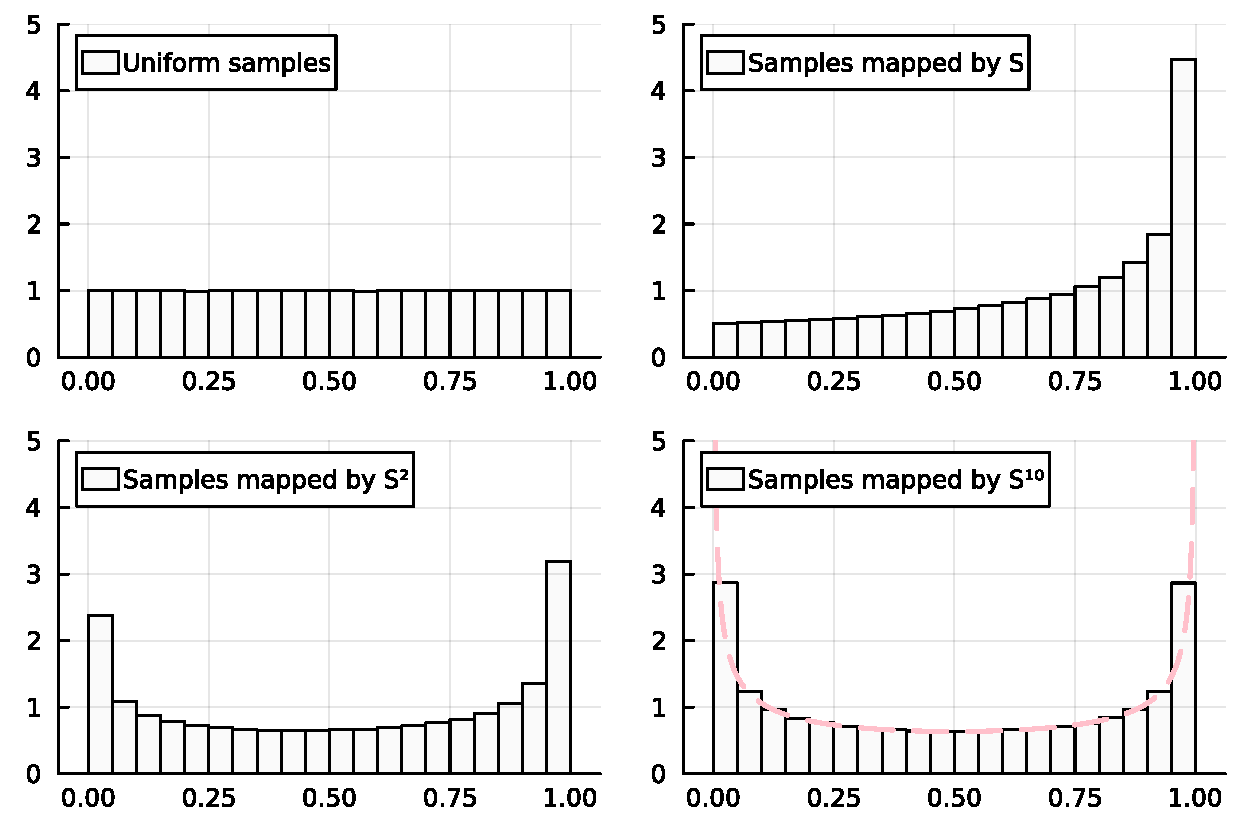
\includegraphics[width=0.85\textwidth]{perron_asymptotic.pdf}
    \caption{
        Illustration of the pushforward intuition of the Perron-Frobenius operator. 
        Action of the $\scrL$ associated with the quadratic map 
        $S : [0, 1] \circlearrowleft,\ x \mapsto 4 x (1 - x)$. One million points are 
        sampled uniformly in $[0, 1]$ and mapped forward under $S$, $S^2$, and $S^{10}$. 
        The respective distributions are shown in histograms. 
    }\label{fig:perron_asymptotic}
\end{figure}

When $S$ is a diffeomorphism, $\scrL$ has an explicit form. 

\begin{theorem}
    Let $S$ be a diffeomorphism. Then 
    \begin{equation}
        \scrL f = \frac{f \circ S^{-1}}{\left| \det D\,S^{-1} \right|}
    \end{equation}
\end{theorem}

In particular one sees that when $S$ is a measure algebra isomorphism (that is, $S$ and 
$S^{-1}$ both preserve the measure) then the Koopman operator is unitary, i.e. 
$\scrK^* (= \scrL) = \scrK^{-1}$. 

\begin{proof}
    This follows from a change of variables $y = S(x)$
    \begin{equation}
        \int g \cdot \scrL f \,dx = \int \scrK \cdot f \,dx 
        = \int f(y) \cdot g \circ S^{-1} (y) \left| \det D\,S (S^{-1} (y)) \right| \,dy . 
    \end{equation}
\end{proof}

\begin{corollary}
    Assume $S$ is a piecewise diffeomorphism, i.e. there exists a disjoint decomposition 
    $\Omega = \biguplus_{l=1}^n U_l$ such that for each $l$, 
    $S_l \defeq \left. S \right|_{U_l} : U_l \to V_l$ is a diffeomorphism. Then 
    \begin{equation}
        (\scrL f) (x) = \sum_{l=1}^{n} 
        \frac{f \circ S_l^{-1} \,(x)}{\left| \det D\,S_l^{-1}\,(x) \right|} \bbone_{V_l} (x) . 
    \end{equation}
\end{corollary}


\subsection{Spectral Properties}

\subsubsection{The Spectrum}

We begin with abstract definitions for parts of the spectrum. 

\begin{definition}
    Let $M : D(M) \to \scrX$ be a linear operator on a Banach space 
    $(X, \| \cdot \|)$. The domain $D(M) \subset \scrX$ of $M$ 
    may be a dense subset of $\scrX$. $M$ is called \emph{closed} if: whenever 
    $x_k \to x$ is a convergent sequence with $M x_k$ convergent, then $M x_k \to M x$. 
\end{definition}

Closedness is weaker than continuity due to the extra assumption that $M x_k$ is 
convergent. 

\begin{definition}
    The \emph{spectrum} $\sigma (M)$ of a closed operator $M$ is the set of numbers 
    $\lambda \in \bbC$ for which $M - \lambda I$ does not have a bounded inverse. The 
    complement $\rho (M) \defeq \bbC \setminus \sigma (M)$ is called \emph{resolvent set} 
    and $( M - \lambda I )^{-1}$ is called the \emph{resolvent}. 
\end{definition}

\begin{proposition}
    The spectrum admits a disjoint decomposition 
    \begin{equation}
        \sigma (M) = \sigma_p (M) \uplus \sigma_c (M) \uplus \sigma_r (M)
    \end{equation}
    into \emph{point-, continuous-,} and \emph{residual-spectrum} with
    \begin{align}
        &\sigma_p (M) = \left\{ \lambda \in \bbC \mid 
            M - \lambda I \text{ is not injective} \right\}, &\phantom{.} \\
        &\sigma_c (M) = \left\{ \lambda \in \bbC \mid 
            M - \lambda I \text{ is injective, but its range is a dense subset of } 
            \scrX \right\}, \\
        &\sigma_r (M) = \left\{ \lambda \in \bbC \mid 
            M - \lambda I \text{ is injective, but does not have dense range} \right\}. 
    \end{align}
\end{proposition}

\begin{remark}
    In some literature, $0$ is never part of the spectrum. We do not take this approach. 
\end{remark}

An element $\lambda \in \sigma_p (M)$ is a \emph{true} eigenvalue in the sense that there 
exists a vector $x \in \scrX$ such that $(M - \lambda I) x = 0$. The continuous spectrum 
has a similar characterization as the set of $\lambda \in \bbC$ for which $M - \lambda I$ 
is injective but \emph{not} bounded from below, i.e. there exists a sequence $(x_k)_k$, 
$\| x_k \| = 1$, for which $0 < \| (M - \lambda I) x_k \| \to 0$. Equivalently, 
$(M - \lambda I)^{-1}$ cannot be extended to a bounded linear operator, but is still a 
(densely defined) closed linear operator. (See the proof of theorem 
\ref{thm:resolvent_adjoint} for a proof of this characterization.)

We have already used the duality pairing \ref{eq:duality} to deduce a form of the 
Perron-Frobenius operator. For completetess we provide a full definition for the adjoint 
of an unbounded operator and cite some basic facts about adjoints. 

\begin{definition}
    \label{thm:adjoint}
    Let $M : \scrX \supset D(M) \to \scrX$ be a densely defined closed linear operator on 
    a Banach space. The \emph{adjoint operator} is constructed as follows. Let 
    \begin{equation}
        D(M^*) = \left\{ f \in \scrX^* \mid \exists\, f' \in \scrX : 
        \left\langle f, M g \right\rangle = \left\langle f', g \right\rangle\ \forall\, 
        g \in D(M) \right\} . 
    \end{equation}
    Now $M^*$ is defined by $M^* f = f'$. 
\end{definition}

\begin{lemma}[\cite{kato}]
    Let $\scrX$ be a reflexive\footnote{
        The bidual $\scrX^{**}$ is isomorphic to $\scrX$, that is, $\scrX^{**} \cong \scrX$. 
    } Banach space. Then the adjoint operator is also densely defined and closed, and
    \begin{enumerate}
        \item $M^{**} = M$,
        \item $\ker (M^*) = \ran (M)^\perp$,
    \end{enumerate}
    where for $A \subset \scrX$, $A^\perp = \left\{ f \in \scrX^* \mid 
    \left\langle f, g \right\rangle = 0\ \forall\, g \in A \right\}$ is the annihilator. 
\end{lemma}

One might ask why such detail is required in defining the spectrum. The answer lies in 
the subtle consequences of infinite-dimensionality. The following example from 
\cite{spectraexample} shows the subtle interplay between residual spectrum and spectrum 
of the adjoint operator, all of which requires infinite-dimensionality. 

\begin{example}[Shift operators on $\ell^2 (\bbN)$]
    \label{ex:shift}
    The canonical right-shift operator

    \begin{equation}
        R : (a_1, a_2, \ldots) \mapsto (0, a_1, a_2, \ldots)
    \end{equation}

    is adjoint to the left shift

    \begin{equation}
        L : (a_1, a_2, \ldots) \mapsto (a_2, a_3, \ldots) . 
    \end{equation}

    We claim: 

    \begin{align}
        \label{eq:pointspec}
        &\sigma_p (L) = \left\{ \lambda \in \bbC \mid | \lambda | < 1 \right\} &
        &\sigma_p (R) = \emptyset \\
        \label{eq:contspec}
        &\sigma_c (L) = \left\{ \lambda \in \bbC \mid | \lambda | = 1 \right\} &
        &\sigma_c (R) = \left\{ \lambda \in \bbC \mid | \lambda | = 1 \right\} \\
        \label{eq:resspec}
        &\sigma_r (L) = \emptyset & 
        &\sigma_r (R) = \left\{ \lambda \in \bbC \mid | \lambda | < 1 \right\} . 
    \end{align}

    Indeed, to see \ref{eq:pointspec} consider $| \lambda | < 1$, 
    $a^\lambda = (\lambda, \lambda^2, \ldots)$. Then clearly 
    $L a^\lambda = \lambda a^\lambda$. On the 
    other hand, suppose $R a = \lambda a$ for some $a \neq 0$, $\lambda \in \bbC$. Then 
    letting $n$ be the first index such that $a_n \neq 0$, we must have 
    $0 = a_{n-1} = (R a)_n = \lambda a_n$ so $\lambda = 0$. But the kernel of $R$ is 
    clearly $\left\{ 0 \right\}$. 

    To see \ref{eq:contspec}, take $| \lambda | = 1$ and construct \emph{approximate} 
    $(L, \lambda)$-eigenvectors 
    $v^n = \left( \lambda, \lambda^2, \ldots, \lambda^n, 0, \ldots \right)$. Then 
    $(L - \lambda I) v^n = (0, \ldots, 0, \lambda^{n+1}, 0, \ldots)$ so 
    $\| (L - \lambda I) v^n \| = 1$ but $\| v^n \| = \sqrt{n}$. It remains to show 
    that $\lambda$ is of continuous spectrum, as opposed to residual spectrum. Indeed, 
    for any $w$ such that for all $v \in \ell^2$, 
    $0 = \left\langle (L - \lambda I) v, w \right\rangle 
    = \left\langle v, (R - \bar{\lambda} I) w \right\rangle$ so that $w$ is an eigenvector of 
    $R$ which by \ref{eq:pointspec} is a contradiction. An entirely analogous argument 
    shows that the circle is also continuous spectrum for $R$. 

    We now reverse the discussion to see that any $| \lambda | < 1$ is in the 
    residual spectrum of $R$. For $v \in \ell^2$ and $w$ a $\bar{\lambda}$-eigenvector of 
    $L$ we have 
    $0 = \left\langle v, 0 \right\rangle 
    = \left\langle v, (L - \bar{\lambda} I) w \right\rangle 
    = \left\langle (R - \lambda I) v, w \right\rangle$ so that the range of 
    $R - \lambda I$ is orthogonal to $w$. 

    Finally, $\sigma (M)$ is bounded by $\| M \|$ for any operator $M$, and clearly 
    $\| L \| = 1$. But $\sigma_p (L) \cup \sigma_c (L) = 
    \left\{ \lambda \in \bbC \mid | \lambda | \leq 1 \right\}$ so 
    $\sigma_r (L) = \emptyset$. Combined with the previous paragraph, this shows 
    \ref{eq:resspec}. 

\end{example}

The example already suggests some important relationships regarding the spectrum of 
adjoint operators. 

\begin{theorem}
    \label{thm:spec_relations_adjoints}
    Let $M$ be a densely defined closed linear operator on a reflexive Banach space. 
    
    \begin{enumerate}
        \item $\lambda \in \sigma (M)$ iff $\bar{\lambda} \in \sigma (M^*)$. 
        \item If $\lambda \in \sigma_r (M)$, then $\bar{\lambda} \in \sigma_p (M^*)$. 
        \item Conversely, if $\lambda \in \sigma_p (M)$, then 
              $\bar{\lambda} \in \sigma_p (M^*) \cup \sigma_r (M^*)$. 
        \item $\sigma_c (M) = \sigma_c (M^*)$. 
    \end{enumerate}
\end{theorem}

\begin{proof}
    \begin{enumerate}
        \item Suppose $M - \lambda I$ has a bounded inverse $B$. Then 
              $(M - \lambda I) B = B (M - \lambda I) = I$. Equivalently 
              $B^* (M^* - \bar{\lambda} I) = (M^* - \bar{\lambda} I) B^* = I^* = I$. 
        \item The range of $M - \lambda I$ is not dense in $\scrX$. Hence there exists a 
              $v \in \text{ran} (M - \lambda I)^\perp$. But this implies 
              $v \in \text{ker} (M^* - \bar{\lambda} I)$. 
        \item There exists a $v \in \text{ker} (M - \lambda I)$ which implies 
              $v \in \text{ran} (M^* - \bar{\lambda} I)^\perp$. 
        \item Follows from $1$, $2$, and $3$. 
    \end{enumerate}
\end{proof}


\subsubsection{Spectra of Koopman and Perron-Frobenius Operators}

The Koopman and Perron-Frobenius operator spectrum holds information about the long-term 
mixing rates of structures in phase space. We write (with some abuse of notation) 
$\left. \scrL \right|_{\scrX}$ and $\left. \scrK \right|_{\scrX}$ to denote the 
Perron-Frobenius / Koopman operators acting on the domain $\scrX$. 

\begin{definition}
    An eigenfunction $f$ for $\left. \scrL \right|_{L^1}$ with eigenvalue $1$ is the 
    density of a \emph{(signed) invariant measure}. We say $S$ \emph{preserves the 
    measure $f\,dx$}. 
\end{definition}

\begin{figure}
    \centering
    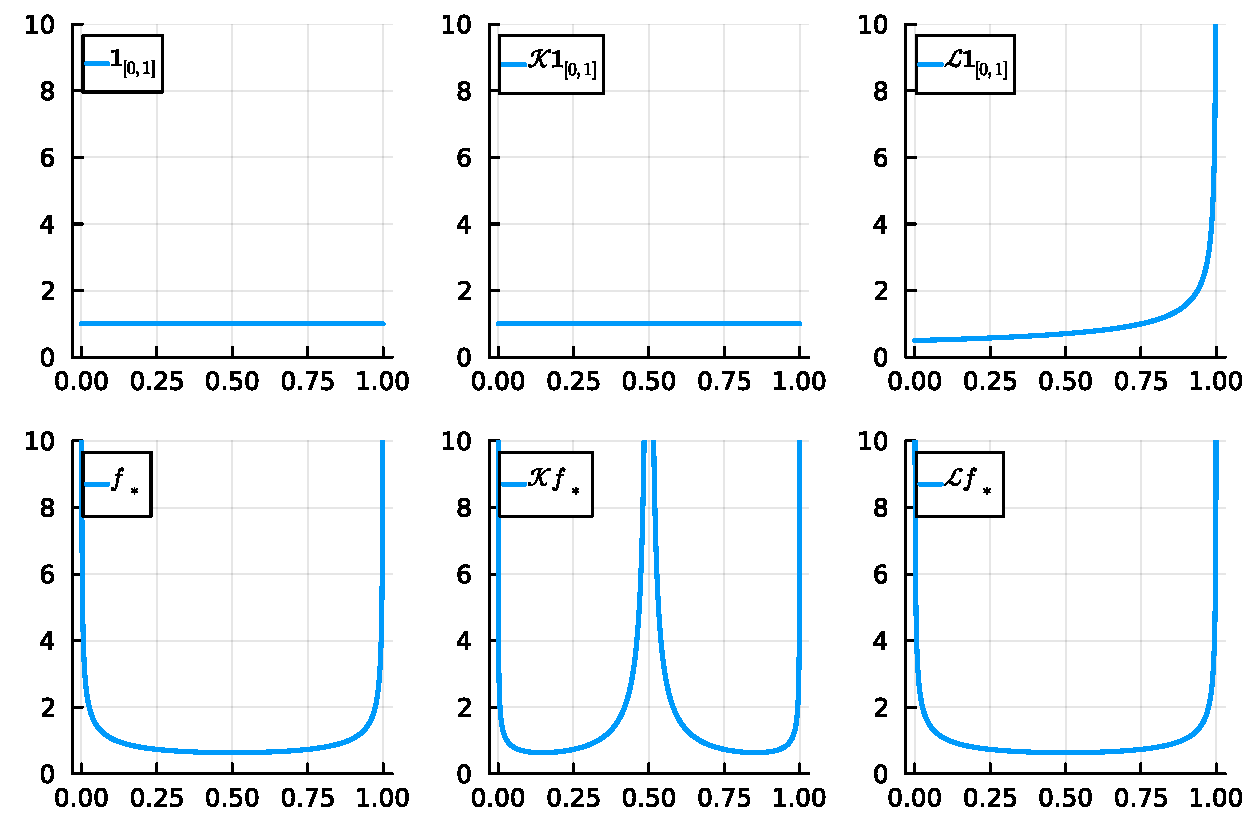
\includegraphics[width=0.9\textwidth]{koopman_perron_invariance_example.pdf}
    \caption{
        Actions of the Koopman and Perron-Frobenius operators associated with the quadratic 
        map $S : [0, 1] \circlearrowleft,\ x \mapsto 4 x (1 - x)$. The constant density 
        $\bbone_{[0, 1]}$ is fixed under $\scrK$ and the density 
        $f_* (x) = \frac{1}{\pi \sqrt{ x (1 - x) }}$ is fixed under $\scrL$ (c.f. figure 
        \ref{fig:perron_asymptotic}). 
    }\label{fig:quadratic_eigs}
\end{figure}

The following are well-known facts about the Koopman and Perron-Frobenius operator. They 
can be found in many sources e.g. \cite{lasotamackey}. 

\begin{theorem}
    \begin{enumerate}
        \item If $S$ is ergodic\footnote{Ergodicity and mixing describe how obeservations 
            become decorrelated over time. $S$ is \emph{ergodic} if for all $A, B \in \scrA$ 
            we have $\frac{1}{n}\sum_{j=0}^{n-1} \int_{ S^{-j} (A) \cap B } dx \to 
            \int_A dx \int_B dx$ as $n \to \infty$. $S$ is weak-mixing if we have 
            $\frac{1}{n}\sum_{j=0}^{n-1} \left| \int_{ S^{-j} (A) \cap B } dx 
            - \int_A dx \int_B dx \right| \to 0$ as $n \to \infty$. },
            then there is at most one invariant density. Conversely, if there is a unique 
            invariant density which is $(dx-)$almost everywhere positive, then $S$ is 
            ergodic. 
        \item If $S$ is ergodic, then every eigenvalue of $\left. \scrK \right|_{L^1}$ 
            is simple. 
        \item Suppose $S$ is invertible. Then $S$ is weak-mixing iff $1$ is the only 
            eigenvalue of $\left. \scrK \right|_{L^1}$. 
    \end{enumerate}
\end{theorem}

The following theorem is from \cite{attr}. 

\begin{definition}
    A set $A \subset \Omega$ in phase space is called \emph{$\delta$-almost-invariant} if 
    \begin{equation}
        \int_{ S^{-1} (A) \cap A } dx = (1 - \delta) \cdot \int_A dx . 
    \end{equation}
\end{definition}

\begin{theorem}
    Let $\bbR \ni \lambda < 1$ be an eigenvalue corresponding to a real-valued 
    normalized eigenfunction $f$ of $\left. \scrL \right|_{L^1}$. Let further 
    $A \subset \Omega$ be such that $\int_A f\, dx = \frac{1}{2}$. Then 

    \begin{equation}
        \delta + \eta = \lambda + 1
    \end{equation}

    if $A$ is $\delta$-almost-invariant and $\Omega \setminus A$ is 
    $\eta$-almost-invariant. 
\end{theorem}

These are only a few interesting properties of the spectrum of these operators, but there 
are many more which can be studied. 


\subsection{Pseudospectra}

The reader will have likely noticed the sensitivity required in understanding the spectrum 
for infinite-dimensional operators. In particular the spectral types can be unstable 
w.r.t. perturbations of the operator. For example, for any self-adjoint operator $M$ (e.g. 
the generator for the Koopman semigroup in a continuous-time dynamical system) there 
exists a compact operator $E$ with arbitrarily small norm such that the perturbation 
$M + E$ has purely point spectrum. 

The situation is even worse when one considers \emph{perturbations of the dynamics} 
instead of perturbations of the Koopman / Perron-Frobenius operators. Consider a circle 
rotation $S : \bbT \to \bbT,\ e^{2\pi i \theta} \mapsto e^{2\pi i (\theta + \alpha)}$. 
We have 
$\sigma ( \left. \scrL \right|_{L^2} ) = \sigma_p ( \left. \scrL \right|_{L^2} ) = \alpha^{\bbN_0}$. 
If the rotation is rational then the spectrum is discrete, but if the rotation is 
irrational then the spectrum is dense in the unit circle. 

In the present paper we tackle the instability problem for operator perturbations. 
One might wonder whether operators which are "close" (in some sense) also have spectra 
which are "close". Unfortunately, this is in general not true. Even in finite dimensions 
this breaks down, as the following example shows. 

\begin{example}[\cite{tao}]
    \label{ex:spec_unstable}
    Let $\scrX = \bbR^n$ and let 
    \begin{equation}
        M = \begin{bmatrix}
            0 &   1    &        &   \\
              & \ddots & \ddots &   \\
              &        &        & 1 \\
              &        &        & 0
        \end{bmatrix} . 
    \end{equation}
    $M$ is nilpotent so $\sigma (M) = \left\{ 0 \right\}$. However, for an arbitrarily 
    small $\epsilon > 0$, the perturbation
    \begin{equation}
        M + E = \begin{bmatrix}
            0        &   1    &        &   \\
                        & \ddots & \ddots &   \\
                        &        &        & 1 \\
            \epsilon &        &        & 0
        \end{bmatrix} . 
    \end{equation}
    has characteristic polynomial $(-\lambda)^n - (-1)^n \epsilon$ so that 
    $\sigma (M + E) = \left\{ \lambda \in \bbC \mid \lambda^n = \epsilon \right\}$. 
    For growing $n$, $\sigma (M + E)$ comes asymptotically close to filling the 
    unit circle. 
\end{example}


\subsubsection{Definitions of the Pseudospectrum}

\begin{definition}
    Let $M : D(M) \to \scrX$ be a closed linear operator. The 
    \emph{$\epsilon$-pseudospectrum} of $M$ is 
    the smallest set in $\bbC$ which contains the spectrum of all perturbations of $M$ 
    with norm less than $\epsilon$:\footnote{
        Some authors will define the pseudospectrum with "$\leq$" instead of "$<$". This 
        makes $\sigma_\epsilon (M)$ a closed set, but breaks theorem \ref{thm:pseudo}.}
    \begin{equation}
        \label{eq:pseudospectrum_union}
        \sigma_\epsilon (M) = \bigcup_{\| E \| < \epsilon} \sigma (M + E). 
    \end{equation}
\end{definition}

\begin{figure}
    \centering
    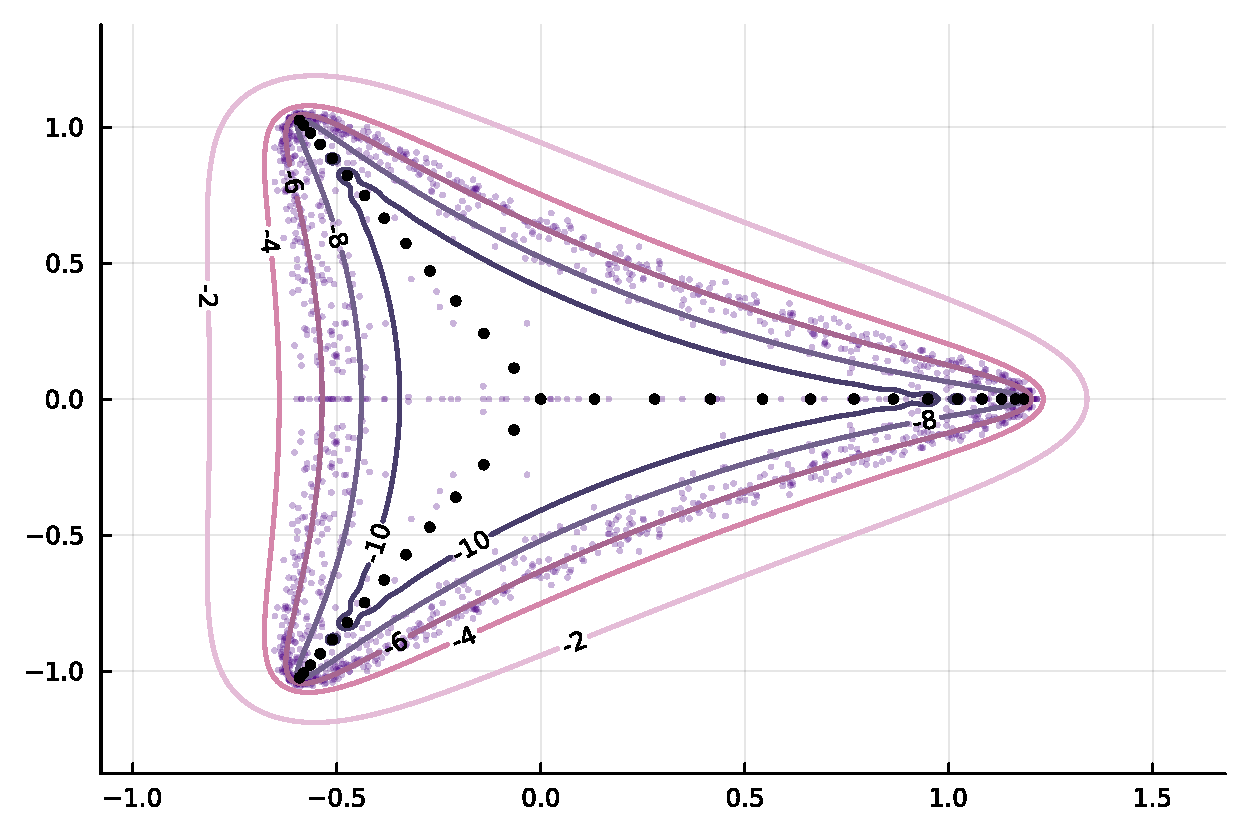
\includegraphics[width=0.8\textwidth]{pseudospectrum_rand.pdf}
    \caption{
        Pseudospectra for the $40 \times 40$ Toeplitz matrix $T$ with $0$ on the main 
        diagonal, $1$ on the first upper off-diagonal, and $1/4$ on the second lower 
        off-diagonal. Contour lines show the boundary of the $\epsilon$-pseudospectrum 
        for $\epsilon = 10^{-2}, 10^{-4}, 10^{-6}, 10^{-8}, 10^{-10}$. Black: Spectrum 
        of $T$. Purple: Spectra of $T + E$ for $40$ randomly sampled 
        perturbations $E$ with $\| E \| < 10^{-4}$. 
    }
\end{figure}

\begin{theorem}
    \label{thm:pseudo}
    We have the following equivalent formulation of the pseudospectrum:
    \begin{equation}
        \sigma_\epsilon (M) = \left\{ \lambda \in \bbC \mid 
        \| (M - \lambda I)^{-1} \| > \frac{1}{\epsilon} \right\} 
    \end{equation}
    where we use the convention that $\| (M - \lambda I)^{-1} \| = \infty$ if 
    $M - \lambda I$ is not invertible. 
\end{theorem}

\begin{remark}
    While this result is practically pseudospectrum folklore, a correct proof in the general 
    case of closed linear operators on Banach spaces is difficult to find. Virtually all 
    sources which cite this result, cite an unpublished technical report by Chaitin-Chatelin 
    and Harrabi \cite{unpublished_pseudospectrum_result}. The following proof is based on 
    \cite{boettcher2005spectral} and extended slightly from bounded operators to closed 
    (potentially) unbounded operators. 
\end{remark}

\begin{proof}
    We prove "$\subset$" by contraposition: assume 
    $\| (M - \lambda I)^{-1} \| > \frac{1}{\epsilon}$ and let $\| E \| < \epsilon$. Then 
    $\| (M - \lambda I)^{-1} E \| < 1$ and hence $I + (M - \lambda I)^{-1} E$ is 
    invertible. This implies 
    \begin{equation}
        M - \lambda I + E 
        = \left( M - \lambda I \right) \left( I + (M - \lambda I)^{-1} E \right)
    \end{equation}
    is invertible. 

    Conversely, we prove "$\supset$" by showing there exists an operator $E$ with 
    $\| E \| < \epsilon$ sich that $M - \lambda I + E$ is not invertible. Since 
    $\| (M - \lambda I)^{-1} \| > \frac{1}{\epsilon}$ there exists a $u \in \scrX$ with 
    $\| u \| = 1$ and $(M - \lambda I)^{-1} u = v \in D(M)$ with 
    $\| v \| = \frac{1}{\delta} > \frac{1}{\epsilon}$.\footnote{
        At this point we require the strict inequality. Otherwise, the existence of such 
        a pair $u$, $v$ is not guaranteed. 
    } The Hahn-Banach theorem provides 
    a $v^* \in \scrX^*$ with $\| v^* \| = 1$ and $v^* v = \| v \| = \frac{1}{\delta}$. 
    Set $E = - \delta u v^*$. Then $\| E \| = \delta < \epsilon$ and 
    \begin{equation}
        E v = - \delta u v^* v = - u = - (M - \lambda I) (M - \lambda I)^{-1} u 
        = - (M - \lambda I) v . 
    \end{equation}
    Rearranging yields $(M + E - \lambda I) v = 0$. 
\end{proof}

The proof of the above theorem also shows that one can consider only rank-one 
perturbations in \ref{eq:pseudospectrum_union}: 

\begin{corollary}
    We can restrict \ref{eq:pseudospectrum_union} to 
    \begin{equation}
        \sigma_\epsilon (M) 
        = \bigcup_{\substack{ \| E \| < \epsilon \\ \text{rank }E = 1 }} 
        \sigma (M + E) . 
    \end{equation}
\end{corollary}

The following formulation of the pseudospectrum in the Hilbert space case will be the 
main tool we use in the section on numerical methods. 

\begin{definition}
    The function 
    \begin{equation}
        \sigma_{\inf} (M) = \inf_{\| x \| = 1} \| M x \|
    \end{equation}
    is known as the \emph{injection modulus}. 
\end{definition}

\begin{lemma}
    \label{lem:injection_modulus}
    Let $M : D(M) \to \scrX$ be a closed linear operator on a Hilbert space. 
    If $\lambda \in \rho (M)$ then 
    \begin{equation}
        \label{eq:injection_modulus_adjoint}
        \sigma_{\inf} (M - \lambda I) = \sigma_{\inf} (M^* - \bar{\lambda} I) , 
    \end{equation}
    but this is \emph{not} necessarily true if $\lambda \in \sigma (M)$. 
\end{lemma}

\begin{proof}
    \ref{eq:injection_modulus_adjoint} for $\lambda \in \rho (M)$ follows from the fact 
    that for bounded operators $A$ we have $\| A \| = \| A^* \|$, applied to 
    $A = (M - \lambda I)^{-1}$. To see that \ref{eq:injection_modulus_adjoint} does not 
    hold for $\lambda \in \sigma (M)$, consider again the right shift from example 
    \ref{ex:shift}. Clearly $\| R x \| = \| x \|$ so $R$ is bounded from below but $0$ 
    is part of the spectrum. 
\end{proof}

\begin{theorem}
    \label{thm:resolvent_adjoint}
    For a Hilbert space operator $M$, 
    \begin{equation}
        \frac{1}{\left\| (M - \lambda I)^{-1} \right\|} = \min \left\{ 
            \sigma_{\inf} (M - \lambda I),\ \sigma_{\inf} (M^* - \bar{\lambda} I)
         \right\} . 
    \end{equation}
    where we use the convention that $1 / \left\| (M - \lambda I)^{-1} \right\| = 0$ 
    when $\lambda \in \sigma (M)$. 
\end{theorem}

\begin{proof}
    When $\lambda \in \sigma_p (M)$, then obviously $\sigma_{\inf} (M - \lambda I) = 0$. 
    Due to theorem \ref{thm:spec_relations_adjoints} part $2$, $\lambda \in \sigma_r (M)$ 
    has $\sigma_{\inf} (M^* - \bar{\lambda} I) = 0$. Finally, let 
    $\lambda \in \sigma_c (M)$ so $M - \lambda I$ is injective. Assume 
    $\sigma_{\inf} (M - \lambda I) > 0$. Then 
    $(M - \lambda I)^{-1} : \text{ran} (M - \lambda I) \to D(M)$ is bounded. 
    But since $\text{ran} (M - \lambda I) \subset \scrX$ is dense, $(M - \lambda I)^{-1}$ 
    has a unique bounded extension to $\scrX$, a contradiction. 
\end{proof}

\begin{corollary}
    \label{cor:pseudospectrum_min_residual}
    In the Hilbert space setting, the psudospectrum can be formulated as: 
    \begin{multline}
        \label{eq:pseudospectrum}
        \sigma_\epsilon (M) = \left\{ \lambda \in \bbC \mid \exists\; u \in \scrX : 
        \| u \| = 1 \text{ and either }\right. \\
        \left.\left\| (M - \lambda I) u \right\| < \epsilon \text{ or } 
        \left\| (M^* - \bar{\lambda} I) u \right\| < \epsilon \right\} .  
    \end{multline}
    In the general Banach space setting,
    \begin{equation}
        \label{eq:pseudospec_min}
        \sigma_\epsilon (M) = \sigma_r (M) \cup \left\{ \lambda \in \bbC \mid \exists\; u \in \scrX : 
        \| u \| = 1,\ \left\| (M - \lambda I) u \right\| < \epsilon \right\} . 
    \end{equation}
\end{corollary}

\iffalse
One sees from the proofs of lemma \ref{lem:injection_modulus} and theorem 
\ref{thm:resolvent_adjoint} that $\sigma (M)$ in equation \ref{eq:pseudospec_min} can be 
replaced with $\sigma_r (M)$. 
\fi
The residual spectrum causes many common and unintuitive 
issues in spectral theory. In the study of pseudospectra, this issue is alleviated in 
one of three ways: $(1)$: consider only classes of operators which have no residual 
spectrum (e.g. finite-dimensional or compact operators), $(2)$: compute a slightly 
different object known as the \emph{approximate-point spectrum} (see below), $(3)$: 
ignore the problem entirely and write proofs which are all slightly incorrect. 

\begin{definition}
    \label{def:approximate_point_spec}
    The \emph{approximate-point pseudospectrum} is the set of points for which there 
    exists an \emph{$\epsilon$-approximate pseudoeigenvector}
    \begin{equation}
        \sigma_{ap, \epsilon} (M) = \left\{ \lambda \in \bbC \mid 
            \exists\; u \in \scrX : \left\| u \right\| = 1,\ 
            \left\| (M - \lambda I) u \right\| < \epsilon 
        \right\} . 
    \end{equation}
    The $\epsilon \to 0$ limit of such sets is the \emph{approximate-point spectrum}
    \begin{align}
        \sigma_{ap} (M) &= \bigcap_{\epsilon > 0} \sigma_{ap, \epsilon} (M) \\
        &= \left\{ \lambda \in \bbC \mid
            \exists\; (u_k)_k : \left\| u_k \right\| = 1\ \forall\; k,\ 
            \lim_{k \to \infty} \left\| (M - \lambda I) u_k \right\| = 0
        \right\} . 
    \end{align}
\end{definition}


\subsubsection{Properties}

To gain some intuition for the pseudospectrum, we derive some properties for specific 
types of operators. 

\begin{definition}
    An operator $M$ on a Hilbert space is called \emph{normal} if $M^* M = M M^*$. 
    Special classes of normal operator include \emph{unitary} operators ($M^* = M^{-1}$) 
    and \emph{self-adjoint} operators ($M^* = M$). 
\end{definition}

\begin{proposition}
    For a normal operator $M$, $\sigma_r (M) = \emptyset$. 
\end{proposition}

\begin{proof}
    Let $\lambda \in \sigma (M)$, $A = M - \lambda I$. If $\lambda$ is not an eigenvalue 
    then $\ker A = \left\{ 0 \right\}$ and 
    \begin{equation}
        \left\{ 0 \right\} = \ker A = \ker A^* = (\text{ran} A)^\perp
    \end{equation}
    where for the second equality we used the normality. Hence $\text{ran} A$ 
    is dense. 
\end{proof}

\begin{lemma}
    \label{lem:resolvent_dist}
    For a closed linear operator $M$ we have
    \begin{equation}
        \label{eq:resolvent_dist}
        \text{dist} (\lambda, \sigma (M)) \geq \frac{1}{
            \left\| (M - \lambda I)^{-1} \right\|} . 
    \end{equation}
    Moreover, if $M$ is a normal operator on a Hilbert space, then we have equality. 
\end{lemma}

\begin{proof}
    Let $\eta \in \sigma (M)$. Denote $A = M - \lambda I$, $B = M - \eta I$. Then $A$ is 
    invertible and 
    \begin{equation}
        \label{eq:resolvent_formula}
        B = A - (A - B) = A (I - A^{-1} (A - B)) . 
    \end{equation}
    Now 
    $\left\| A^{-1} (A - B) \right\| \leq \left\| A^{-1} \right\| \left| \lambda - \eta \right|$
    so if $| \lambda - \eta | < \frac{1}{\left\| B^{-1} \right\|}$ then the right hand 
    side of \ref{eq:resolvent_formula} is invertible, a contradiction to 
    $\eta \in \sigma (M)$. 

    To prove equality in the case of normal operators requires some heavy machinery from 
    operator theory, namely:
    \begin{enumerate}
        \item Every normal operator is unitarily similar to a multiplication operator 
            on some semi-finite measure space (i.e. there exists a unitary $U$ such that 
            $M = U^{-1} M_a U$ where $(M_a f) (x) = a(x) f(x)$ is a multiplication 
            operator). 
        \item For multiplication operators, equation \ref{eq:resolvent_dist} holds with 
            equality. 
    \end{enumerate}
    These results can be found in many sources e.g. \cite{barrysimon}. 
\end{proof}

\begin{theorem}
    \label{thm:pseudospectrum_growth}
    We have
    \begin{enumerate}
        \item $\sigma_\delta (M) \subset \sigma_\epsilon (M)$ whenever $\delta \leq \epsilon$,
        \item $\bigcap_{\epsilon > 0} \sigma_\epsilon (M) = \sigma (M)$,  
        \item $\sigma (M) + B_\epsilon \subset \sigma_\epsilon (M)$, where $B_\epsilon$ is 
            the ball with radius $\epsilon$ centered at $0$ and $+$ refers to pointwise 
            summation $C + D = \left\{ x + y \mid x \in C,\ y \in D \right\}$. 
        \item When $M$ is normal, $\sigma (M) + B_\epsilon = \sigma_\epsilon (M)$. 
    \end{enumerate}
\end{theorem}

\begin{remark}
    Theorem \ref{thm:pseudospectrum_growth} effectively says that the Pseudospectra are 
    nested sets which grow \emph{at least} as quickly as $\epsilon$-balls around the 
    spectrum. 
\end{remark}

\begin{proof}
    $1$ and $2$ are consequences of the representation \ref{eq:pseudospectrum_union} of 
    the pseudospectrum. $3$ and $4$ are consequences of lemma \ref{lem:resolvent_dist}. 
\end{proof}

We will use the following theorem from Globevnik \cite{globevnik} and Daniluk 
\cite{daniluk}, the proof of which if not very instructive. 

\begin{lemma}
    \label{lem:resolvent_norm_nonconst}
    Let $M$ be a bounded linear operator on a Hilbert space $\scrX$. 
    Then the resolvent norm cannot be constant on an open set. 
\end{lemma}

This lemma can be extended to $L^p$ spaces \cite{wienerhopf}, finite dimensional 
Banach spaces \cite{Harrabi}, Banach spaces which are complex uniformly convex 
\cite{globevnik}, but \emph{not} general infinite dimensional Banach spaces 
\cite{Shargorodsky}. 

\begin{theorem}
    \label{thm:pseudospectrum_continuous}
    The function which maps $(\epsilon, M) \mapsto \sigma_\epsilon (M)$ which sends an 
    $\epsilon > 0$ and a bounded $M$ acting on a Hilbert space $\scrX$ to the set 
    $\sigma_\epsilon (M)$ is continuous using the metric 
    \begin{equation}
        d(\, (\epsilon_1, M_1),\ (\epsilon_2, M_2) \,) 
        = | \epsilon_1 - \epsilon_2 | + \left\| M_1 - M_2 \right\|
    \end{equation}
    in the domain and the Haussdorff metric in the codomain. 
\end{theorem}

\begin{remark}
    \begin{enumerate}
        \item The idea for the proof is taken from
        \cite{pseudospectrum_continuous}, though it originally included two
        errors: it does not take into account residual spectrum, and makes a
        bound which is unfortunately not correct. These issues can be lifted in
        the Hilbert space setting, so that the theorem is still correct as it is
        stated in \cite{pseudospectrum_continuous}. 
        \item If one replaces $\sigma_\epsilon (M)$ with $\sigma_{ap, \epsilon}
        (M)$ in theorem \ref{thm:pseudospectrum_continuous}, then the proof in
        \cite{pseudospectrum_continuous} is essentially correct (save for the 
        bound) and even works for any space where the resolvent norm cannot be 
        constant. To the best of this author's knowledge, there is no
        published correct proof for the general Banach space setting with 
        $\sigma_\epsilon (M)$, despite it being
        considered common knowledge in the study of pseudospectra. 
    \end{enumerate}
\end{remark}

\begin{proof}
    Let $(M, \epsilon)$ and $(M', \epsilon')$ be such that 
    $d\left(\, (M, \epsilon),\ (M', \epsilon') \,\right) < \delta$ for some 
    $0 < \delta < \epsilon / 2$. Without loss of generality let 
    $\epsilon \leq \epsilon'$. 
    
    Let $\lambda \in \sigma_{\epsilon'} (M')$. By 
    \ref{eq:pseudospectrum} there exists a normalized $v \in \scrX$ such that 
    either $\left\| (M' - \lambda I) v \right\| < \epsilon'$ or 
    $\left\| (M'^* - \bar{\lambda} I) v \right\| < \epsilon'$. Assume the former is true. 
    It follows
    \begin{equation}
        \label{eq:M_Mprime}
        \left\| (M - \lambda I) v \right\| 
        \leq \left\| (M - M') v \right\| + \left\| (M' - \lambda I) v \right\|
        < \delta - \left| \epsilon - \epsilon' \right| + \epsilon'
        \leq \delta + \epsilon
    \end{equation}
    where for the last inequality we used that 
    $\epsilon \geq \epsilon' - \left| \epsilon' - \epsilon \right|$. By 
    \ref{eq:pseudospectrum}, $\lambda \in \sigma_{\epsilon + \delta} (M)$ and hence 
    $\sigma_{\epsilon'} (M') \subset \sigma_{\epsilon + \delta} (M)$. 
    
    For the case that 
    $\left\| (M'^* - \bar{\lambda} I) v \right\| < \epsilon'$, equation \ref{eq:M_Mprime} 
    can be done exactly the same with $\left\| (M^* - \bar{\lambda} I) v \right\|$ on 
    the left hand side. 

    Now let $\lambda \in \sigma_{\epsilon - \delta} (M)$. Again this implies there exists 
    a normalized $v \in \scrX$ such that either 
    $\left\| (M - \lambda I) v \right\| < \epsilon - \delta$ or 
    $\left\| (M^* - \bar{\lambda} I) v \right\| < \epsilon - \delta$. Assume again the 
    former is true. Then 
    \begin{equation}
        \left\| (M' - \lambda I) v \right\| 
        \leq \left\| (M' - M) v \right\| + \left\| (M - \lambda I) v \right\|
        < \delta + \epsilon - \delta
        \leq \epsilon'
    \end{equation}
    and hence $\lambda \in \sigma_{\epsilon'} (M')$ so that 
    $\sigma_{\epsilon - \delta} (M) \subset \sigma_{\epsilon'} (M')$ (again the adjoint 
    case can be done exactly the same with adjoints on the left hand side of the equation). 

    We now have 
    $\sigma_{\epsilon - \delta} (M) 
    \subset \sigma_{\epsilon'} (M') 
    \subset \sigma_{\epsilon + \delta} (M)$
    which implies for the Haussdorff distance between $\sigma_\epsilon (M)$ and 
    $\sigma_{\epsilon'} (M')$,
    \begin{align}
        \scrH & \left(\, \sigma_\epsilon (M),\ \sigma_{\epsilon'} (M') \,\right) \\
        & \leq \max \left\{\,
            \scrH \left(\, \sigma_\epsilon (M),\ \sigma_{\epsilon - \delta} (M) \,\right),\ 
            \scrH \left(\, \sigma_\epsilon (M),\ \sigma_{\epsilon + \delta} (M) \,\right) 
        \,\right\} \\
        & \leq \scrH \left(\, 
            \sigma_{\epsilon - \delta} (M),\ 
            \sigma_{\epsilon + \delta} (M) 
        \,\right) . \label{eq:hauss_epsilon_delta}
    \end{align}
    Appealing to lemma \ref{lem:resolvent_norm_nonconst} now yields the claim. 
    \iffalse
    so we must investigate the difference between $\sigma_{\epsilon - \delta} (M)$ and 
    $\sigma_{\epsilon + \delta} (M)$. But 
    \begin{equation}
        \label{eq:epsilon_delta_diff}
        \sigma_{\epsilon + \delta} (M) \setminus \sigma_{\epsilon - \delta} (M) 
        = \left\{ \lambda \in \bbC \mid 
            \frac{1}{\epsilon + \delta}
            < \left\| (M - \lambda I)^{-1} \right\| 
            < \frac{1}{\epsilon - \delta}
        \right\}
    \end{equation}
    which is just a difference of sublevel sets for the continuous function 
    $\lambda \mapsto \left\| (M - \lambda I)^{-1} \right\|$. Hence 
    \ref{eq:epsilon_delta_diff} collapses continuously to $\emptyset$ as $\delta \to 0$, 
    which implies \ref{eq:hauss_epsilon_delta} converges to $0$ as $\delta \to 0$. 
    \fi
\end{proof}

We conclude the section on mathematical background by examining the interaction between 
an operator and finite rank approximations of it. The methods we will describe in the 
following section are special types of \emph{finite-section methods}. 

\begin{theorem}
    \label{thm:projection_pseudospectrum}
    Let $M$ be a closed linear operator and $\left( \Pi_n : \scrX \to V_n \right)_n$ be 
    a collection of projections onto finite-dimensional subspaces $V_n$ which converge 
    pointwise to the identity. Let further $(\lambda, c)$ be an 
    $\epsilon$-pseudoeigenpair of $\Pi_n M \Pi_n$. Then for every $\delta > 0$ 
    there exists an $N = N(\delta, c)$ such that 
    $\lambda \in \sigma_{\epsilon + \delta} (M)$ whenever $n > N$. 

    However, this does \emph{not} necessarily imply 
    $\sigma_\epsilon (\Pi_n M \Pi_n) \to \sigma_\epsilon (M)$ in the Haussdorff metric. 
\end{theorem}

\begin{proof}
    Let $N$ be such that of off-diagonal action of $(M - \lambda I)$ on $c$ is bounded by 
    $\delta$, i.e. $\left\| (I - \Pi_N) (M - \lambda I) \Pi_N c \right\| < \delta$. Now 
    the claim follows from the triangle inequality since
    \begin{equation}
        (M - \lambda I) c = (\Pi_N M \Pi_N - \lambda I) c + (I - \Pi_N) (M - \lambda I) \Pi_N c
    \end{equation}
    and (by definition) $c = \Pi_N c$. 

    For the second claim of the theorem consider the \emph{two-sided} left shift 
    operator $L : \ell^2 \to \ell^2$ and let 
    \begin{equation}
        \Pi_n : (\ldots, a_{-1}, a_0, a_1, \ldots) \mapsto 
        (\ldots, 0, 0, a_{-n}, \ldots a_{-1}, a_0, a_1, \ldots, a_n, 0, 0, \ldots) . 
    \end{equation}
    Then $L$ is unitary and has spectrum on the (complex) unit circle $\bbT$, so 
    $\sigma_\epsilon (L) = \bbT + B_\epsilon$. However, $\Pi_n L \Pi_n$ is nilpotent 
    so $\sigma_\epsilon (\Pi_n L \Pi_n)$ always contains $0$, which is not in 
    $\bbT + B_\epsilon$ for any $\epsilon < 1$. 
\end{proof}


With an understanding of the spectral properties of Koopman and Perron-Frobenius operators 
as well as the pseudospectrum, we are prepared to apply pseudospectral methods to some of 
the most common Koopman approximation methods, known under the umbrella term 
\emph{dynamic mode decomposition}. 


% -------------------------------------------------------------------------------------- %
